% !TEX encoding = UTF-8 Unicode
\documentclass{report}
\title{Practica 3}
\author{Rafael Leyva}
\date{\today}
	
% big font for sections
\usepackage{sectsty}
\sectionfont{\LARGE}
\usepackage[utf8]{inputenc}
\usepackage{graphicx}
\usepackage{wrapfig}
\usepackage{caption}
\usepackage{subcaption}
\usepackage{listings}
\usepackage{hyperref}
\usepackage{float}

% \begin{comment} ... \end{comment{}
\usepackage{verbatim}

\setlength{\parskip}{0pt}
%localizacion de las imagenes
%\graphicspath{ {images/} }

\makeatletter
\renewcommand{\paragraph}{
  \@startsection{paragraph}{4}
    {\z@}{1.25ex \@plus 1ex \@minus .2ex}{-1em}
      {\normalfont\normalsize\bfseries}
      }
      \makeatother

\usepackage[
	sorting=none,
	minbibnames=8,
	maxbibnames=9,
	block=space,
	backend=biber
]{biblatex}
\bibliography{publications}


\usepackage{parskip}

\begin{document}

\newpage

\maketitle

\newpage

\renewcommand{\contentsname}{Indice de contenidos}
\tableofcontents


%=================
\section{Introducción}
	Memoria sobre la realización de la tercera practica de la asignatura Inteligencia Artificial del grado en Ingenieria Informatica en la Universidad de Granada.

	La practica 3 consistente en busqueda en espacios de estados para juegos con informacion perfecta para dos jugadores ha consistido en la implementacion de una variante del clásico juego 4 en raya llamado "Desconecta 4" en el cual el jugador que gana es el que consigue que su oponente conecte 4 fichas en linea (justo al contrario que en la version clásica del juego) con la particularidad de introducir una ficha boomba que elimina las fichas del color del jugador que la detona que esten en su misma fila.

	Para la realizacion ha sido necesario implementar un algoritmo de poda Alfa-Beta para la exploración del arbol de estados del juego asi como una heuristica de valoración de los diferentes estados que es la usada como criterio para  podar en dicho arbol.

\section{Realizacion de la poda Alfa-Beta}
\label{sec:poda}

	La realización del algoritmo de poda ha sido implementado como una clase que no es miembro de la clase player que es la que estamos modificando para esta practica.

	El algoritmo genera los descendientes del tablero actual que es pasado como parametro y evalua la función heuristica para cada uno de dichos hijos, devolviendo en función del tipo de nodo (Min o Max) la valoracion correspondiente.

	Dentro de la funcion de poda el parametro mas destacado es 'acc', un entero pasado por referencia que almacenara la acción que ha obtenido una mayor valoracion en la poda Alfa-Beta. Dicho parametro es usado en el metodo de la clase player Think para aplicar la siguiente acción al tablero y asi intentar alcanzar nuestro objetivo de ganar la partida.

\section{Valoracion heuristica}
\label{sec:heuristica}

\subsection*{Heuristica 1}
	La función heuristica realizada para la valoración de los distintos tableros consiste en aplicar una valoración positiva a todas las conexiones que tiene el jugador contrario, de tal modo que:

	\begin{itemize}
		\item Cada tres fichas conectadas suman 1000.
		\item Cada dos fichas conectadas suman 100.
		\item Que el jugador contrario tenga la bomba en el tablero suma 100.
	\end{itemize}

	Y para el jugador que maneja la IA la heuristica se conforma de la siguiente forma:
	
	\begin{itemize}
		\item Cada tres fichas conectadas resta 100.
		\item Cada dos fichas conectadas resta 10.
		\item Tener la bomba resta 500 al total de la heurística.
	\end{itemize}

	Consiguiendo que la IA se mueva hacia situaciones en las que el contrario tenga muchas fichas conectadas aun a costa de tener fichas conectadas propias, en este sentido la IA es poco conservadora. Además primara las casillas en las que la bomba de la propia IA haya sido detonada de tal forma que el jugador contrario consiga más conexiones.

\subsection*{Heuristica 2}
	Como segunda propuesta a la heurística anteriormente comentada se añadio a la valoracion la opcíón de tener en cuenta los cuadrados de 3x3 fichas que hay en el tablero de juego, con lo que la valoracion heuristica queda de la siguiente forma:

	\begin{itemize}
		\item Cada tres fichas conectadas suman 1000.
		\item Cada dos fichas conectadas suman 100.
		\item Que el jugador contrario tenga la bomba en el tablero suma 100.
		\item Cada cuadrado de 3x3 fichas juntas del rival tambien me beneficia.
	\end{itemize}

	Y para el jugador que maneja la IA la heuristica se conforma de la siguiente forma:
	
	\begin{itemize}
		\item Cada tres fichas conectadas resta 100.
		\item Cada dos fichas conectadas resta 10.
		\item Tener la bomba resta 500 al total de la heurística.
		\item tener juntas 3x3 fichas suma 100 por cada cuadrado de 3x3.
	\end{itemize}

	Aparte de conseguir los mismos resultados de agresividad que en la heuristica 1, esta modificacion ha sido util para evitar tener muchas fichas juntas, lo cual es potencialmente peligroso.

% we use input to include the conclusion, in order to
% get the bibliography and conclusion on the same page
\section{Experimentos}
\label{sec:experimentos}
	A continuacion como resultado se muestran algunas imagenes de partidas jugadas contra la propia heuristica, el jugador ninja y un jugador humano. Los tres `Jugadores'  citados anteriormente juegan con las fichas azules, es decir cada vez que se ve el mensaje `GANA EL JUGADOR VERDE' es la IA programada en esta practica la que vence.


	Partida en la que se ha probado la heuristica 1 programada jugando contra ella misma:

		\begin{figure} [H]
			\begin{center}
				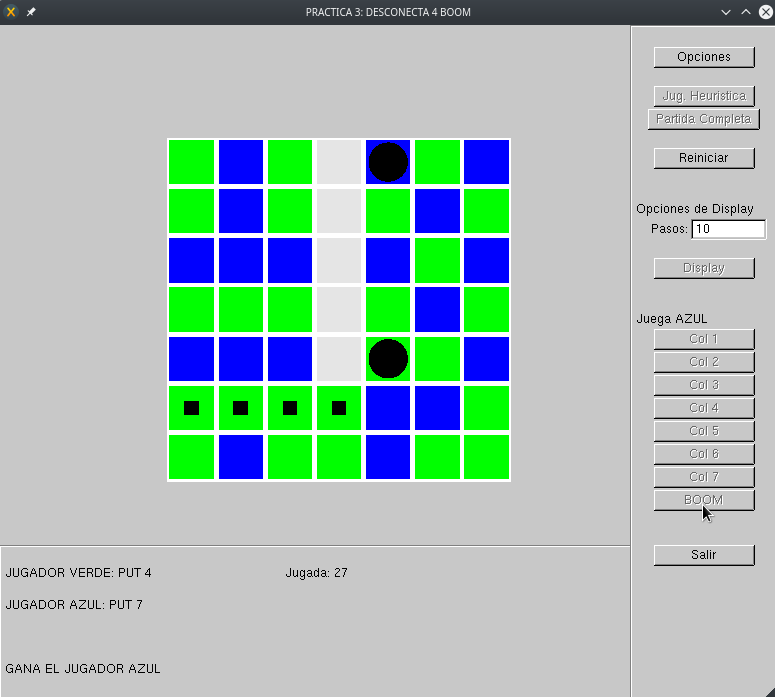
\includegraphics[width=9cm]{HeurVSHeur}
				\caption{Captura de la partida Heur Vs Heur}
				\label{uno}
			\end{center}
		\end{figure}

 	A continuación se muestra una partida contra el jugador ninja que se supone tiene buena heuristica implementada:

 	\begin{figure}[H]
 		\begin{center}
		 	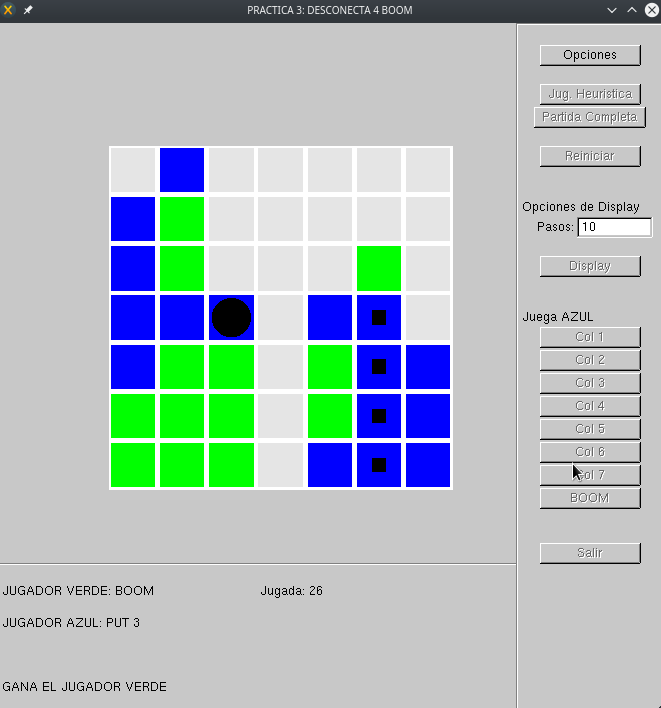
\includegraphics[width=9cm]{HeurVSNinja.png}
		 	\caption{Captura de la partida Heuristica VS Ninja}
		 	\label{dos}
 		\end{center}
 	\end{figure}


 	Y una partida contra el jugador ninja en la que la IA es el  jugador 2 (AZUL).

 	\begin{figure}[H]
		\begin{center}
	 	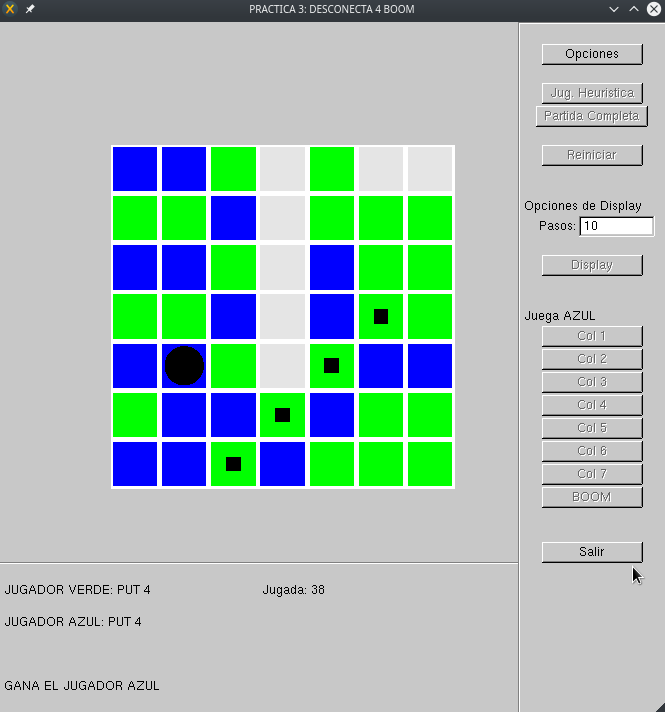
\includegraphics[width=9cm]{NinjaVSHeur.png}
	 	\caption{Captura de la partida Heuristica VS Ninja}
	 	\label{dos}
		\end{center}
	\end{figure}

	Con la segunda heuristica se ha obtenido un 100\% de exito en las partidas contra el jugador ninja.

 %	Partida jugada contra un jugador humano:

% 	\begin{figure}[H]
%	 	\includegraphics[width=10cm]{HeurVSHuman}
%	 	\caption{Captura de la partida Heuristica VS Humano}
%	 	\label{tres} 
% 	\end{figure}



%

%%=================
%\section{Bibliography}
%\label{bib}%

%% \nocite is used to display all references from publications.bib -- even
%% if they were not cited. 
%\nocite{*} %

%\printbibliography[heading=none]%

\end{document}
